\documentclass[12pt,a4paper]{report}

%% Vložení užitečných balíčků
% Geometry and page layout
\usepackage[left=3cm,right=3cm,top=3cm,bottom=3cm]{geometry}

% Fonts and locale
\usepackage{fontspec}
% \usepackage[czech]{babel}
\setmainfont{Geist.ttf}[
  Path = ./assets/fonts/,        % Adjust path to your font directory
  Extension = .ttf,
  UprightFont = *-Regular,
  BoldFont = *-Bold,
]


% Document enhancements
\usepackage[pdfa, colorlinks=false, urlcolor=black, bookmarksopen=true]{hyperref}
\usepackage[backend=biber, style=iso-numeric]{biblatex}
\usepackage{titlesec}

% Graphics and tables
\usepackage{graphicx, xcolor, booktabs, wrapfig}
\graphicspath{{98-images/}}
\usepackage{pgfplots}
\pgfplotsset{compat=1.18}
\usetikzlibrary{arrows}

% Text and math formatting
\usepackage{amsmath, bm, mathrsfs}
\usepackage{microtype, paralist, enumitem, fancyvrb, indentfirst, tocbibind, float, cancel, ragged2e, dcolumn}
\usepackage{needspace, subcaption}

\justifying

% Miscellaneous
\usepackage{lipsum} % For placeholder text


%% Definice různých užitečných maker (viz popis uvnitř souboru)

\DefineBibliographyStrings{czech}{ % Definování vlastního názvu pro bibliografii v češtině
  bibliography = Seznam použité literatury,
}

% TODO
\newcommand{\todo}[1]{\textcolor{red}{(\noindent TODO: #1.)}}

% Celá jména
\newcommand{\name}[1]{\mbox{\textsc{#1}}}

% Cesty
\newcommand{\appendixpath}{components/appendix}

% Images
\newcommand{\subfigwidth}{6cm}        % šířka okénka pro "podobrázky"
\newcommand{\wrappedfigwidth}{6cm}
\newcommand{\fullhd}{0.2}             % měřítko Full HD obrázku
\newcommand{\normalipe}{0.8}          % standardní měřítko IPE obrázku
\newcommand{\fractalscale}{0.3}       % měřítko obrázku softwarem vygenerovaného fraktálu

%%% Prostředí pro sazbu kódu, případně vstupu/výstupu počítačových
%%% programů. (Vyžaduje balíček fancyvrb -- fancy verbatim.)

\DefineVerbatimEnvironment{code}{Verbatim}{fontsize=\small, frame=single}

% Zapne černé "slimáky" na koncích řádků, které přetekly, abychom si
% jich lépe všimli.
\overfullrule=1mm

% Trochu volnější nastavení dělení slov, než je default.
\lefthyphenmin=2
\righthyphenmin=2

\setlength{\parskip}{0.3em}

% Customizing chapters to have a specific look
\titleformat{\chapter}
  {\normalfont\huge\bfseries}{\thechapter.}{1em}{}

% Customizing sections similarly
\titleformat{\section}
  {\normalfont\Large\bfseries}{\thesection}{1em}{}

\makeatletter
\newcommand\openright{\cleardoublepage}
\makeatother




%%% Údaje o~práci

%%% Název práce v~jazyce práce (přesně podle zadání)
\def\NazevPrace{OLAP a ClickHouse}

%%% Název práce v~angličtině
\def\NazevPraceEN{\todo{Title}}

%%% Typ práce
\def\TypPrace{Seminární práce}

%%% Jméno autora
\def\AutorPrace{Martin Kopecký}



%%% Rok odevzdání
\def\RokOdevzdani{2024}

% Studijní program a~obor
\def\StudijniProgram{Aplikovaná informatika}
\def\StudijniObor{Informační systémy}


%%% 3 až 5 klíčových slov (doporučeno), každé uzavřeno ve složených závorkách
\def\KlicovaSlova{%
{}, {klicova slova}
}
%\def\KlicovaSlovaEN{%
%{keywords}
%}

%%% Balíček hyperref, kterým jdou vyrábět klikací odkazy v~PDF,
%%% ale hlavně ho používáme k~uložení metadat do PDF (včetně obsahu).
%%% Většinu nastavítek přednastaví balíček pdfx.
\hypersetup{unicode}
\hypersetup{breaklinks=true}


\renewcommand{\bibname}{Seznam použité literatury}
\addbibresource{./literature/literature.bib}

%% Titulní strana a~různé povinné informační strany
\begin{document}
%%% Titulní strana práce a další povinné informační strany

%%% Titulní strana práce

\pagestyle{empty}
\hypersetup{pageanchor=false}

\begin{center}

%\centerline{\mbox{
\includegraphics[width=166mm]{components/images/ujep.png}}}
\null


{\bf\Large Univerzita Jana Evangelisty Purkyně \\ v Ústí nad Labem}

\vspace{2mm}

{\bf\Large Přírodovědecká fakulta}

\vspace{20mm}


\includegraphics[width=80mm]{ujep.png}

\vspace{20mm}


{\LARGE\bfseries\NazevPrace}

{\large\bfseries\TypPrace}

\vfill


\begin{flushleft}
\begin{tabular}{>{\bfseries}r l}
    \textbf{Vypracoval:} & \AutorPrace \\
    % Vedoucí práce:\Vedouci 
    % Konzultant: \Vedouci
    \\

    \textbf{Studijní program:}  &  \StudijniProgram \\
    \textbf{Studijní obor:}  &   \StudijniObor \\
\end{tabular}
\end{flushleft}

\vfill

% Zde doplňte rok
\large{Ú\raisebox{-0.75ex}{\textsuperscript{STÍ NAD}} L\raisebox{-0.75ex}{\textsuperscript{ABEM}} \RokOdevzdani}

\end{center}

\newpage

\openright
\pagestyle{plain}
\pagenumbering{arabic}
\setcounter{page}{1}

%%% Strana s automaticky generovaným obsahem bakalářské práce

\tableofcontents

%%% Jednotlivé kapitoly práce jsou pro přehlednost uloženy v~samostatných souborech
\chapter{Výběr vhodného DBMS}
Na návrh ostatních kolegů jsem si vybral ClickHouse. Při srovnání různých databázových systémů jsem dospěl k názoru, že výběr správného DBMS pro moje potřeby není zásadně důležitý. ClickHouse mi však umožnil úspěšně zvládnout téměr všechny zadané úkoly. Jediný úkol který jsem nebyl schopen udělat bylo udělání data miningu nad daty.
\chapter{Čištění datasetu}
Protože jsem měl štěstí při výběru datasetu, tak jsem měl již čistá data v datasetu.

\section{Datová kostka}
Při pohledu na data jsem se rozhodlo pro použití schématu hvězdy. Kdy jsem dataset rozdělil na jednotlivé dimenze. Nakonec jsem skončil u 3 dimenzí (Čas, Lokace, Majetek), které spolu svazuje klíčová tabulka.

\vspace{1cm}

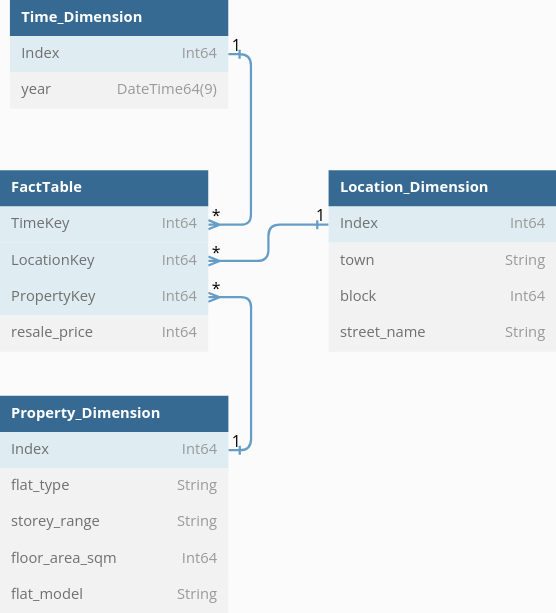
\includegraphics[width=120mm]{kostka.png}

\section{Datová kostka}
Po rozdělení datasetu do dimenzí vypadají jednotlivé dimenze zhruba takto

\subsection{Location\_Dimension}
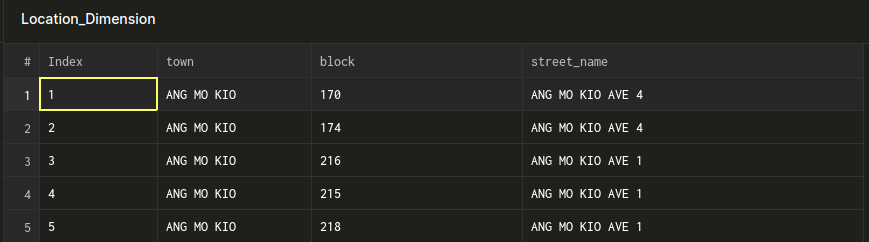
\includegraphics[width=140mm]{Location.png}

\subsection{Time\_Dimension}
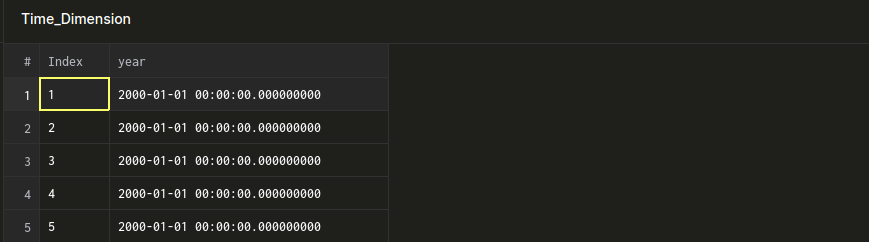
\includegraphics[width=140mm]{Time.png}

\subsection{Property\_Dimension}
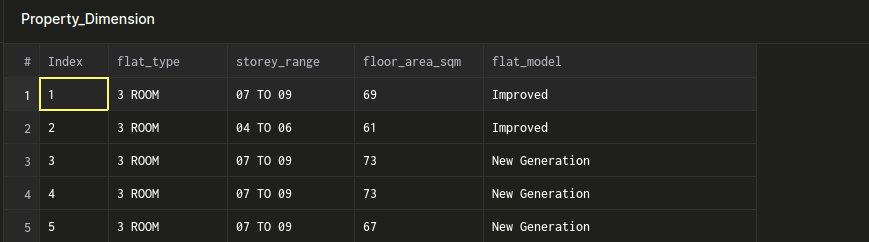
\includegraphics[width=140mm]{Property.png}
\chapter{Jednotlivé řezy kostky}

\section{Ceny bytů napříč roky - rozděleny podle typu}

\begin{lstlisting}[
           language=SQL,
           showspaces=false,
           basicstyle=\ttfamily,
           commentstyle=\color{gray},
           keywordstyle=\color{cyan}
        ]
SELECT 
    toYear(Time_Dimension.year) as Rok, 
    avgIf(resale_price, flat_type = '1 ROOM') as `1-room`, 
    avgIf(resale_price, flat_type = '2 ROOM') as `2-room`, 
    avgIf(resale_price, flat_type = '3 ROOM') as `3-room`, 
    avgIf(resale_price, flat_type = '4 ROOM') as `4-room`, 
    avgIf(resale_price, flat_type = '5 ROOM') as `5-room`, 
    avgIf(resale_price, flat_type = 'MULTI-GENERATION') 
        as `Multi-generation`, 
    avgIf(resale_price, flat_type = 'EXECUTIVE') 
        as `executive` 
FROM 
    FactTable 
JOIN 
    Property_Dimension ON 
        Property_Dimension.Index = FactTable.PropertyKey 
JOIN 
    Time_Dimension ON 
        Time_Dimension.Index = FactTable.TimeKey 
GROUP BY 
    Rok;
\end{lstlisting}

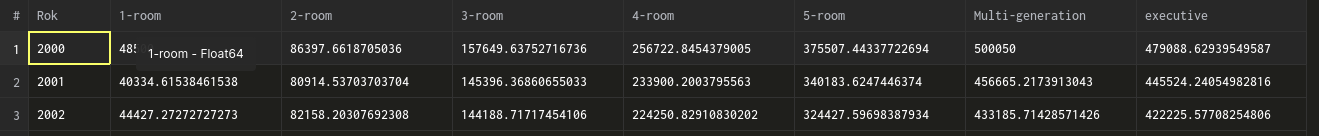
\includegraphics[width=150mm]{priceperyear-data.png}

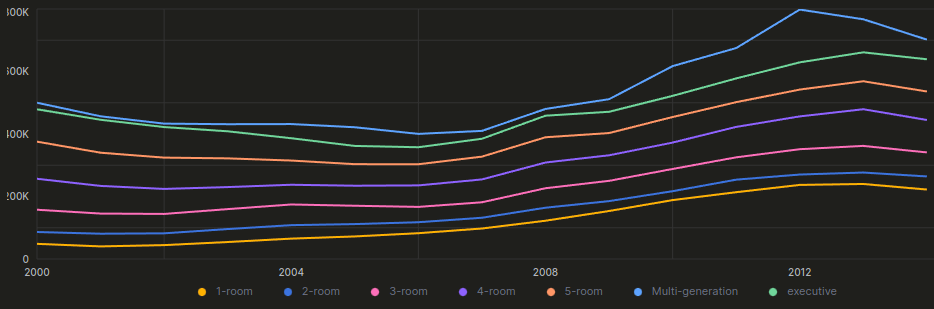
\includegraphics[width=150mm]{priceperyear.png}



\newpage
\section{Nejvyšší cena bytu - rozděleno na typy}

\begin{lstlisting}[
           language=SQL,
           showspaces=false,
           basicstyle=\ttfamily,
           commentstyle=\color{gray},
           keywordstyle=\color{cyan}
        ]
SELECT 
    flat_type, MAX(resale_price) 
        as highest_resale_price 
FROM 
    FactTable 
JOIN 
    Property_Dimension ON 
        FactTable.PropertyKey = Property_Dimension.Index 
GROUP BY 
    flat_type;
\end{lstlisting}

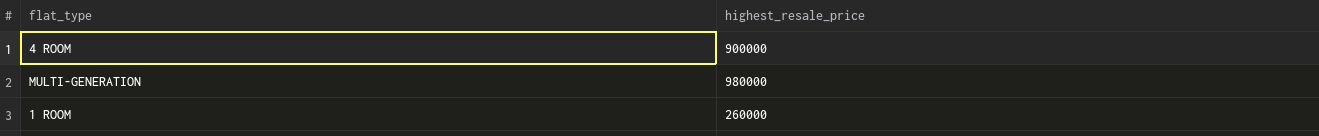
\includegraphics[width=150mm]{hvalpertype-data.png}

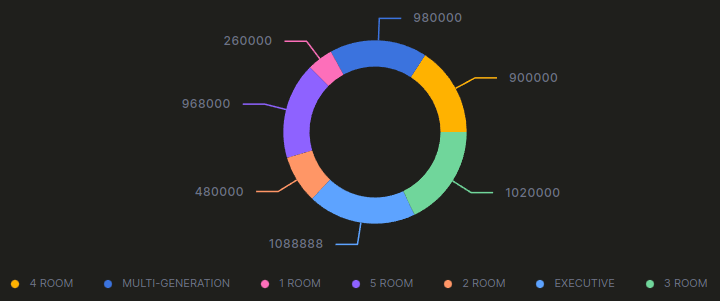
\includegraphics[width=150mm]{hvalpertype.png}


\newpage
\section{Průměrná cena bytů - na časové ose}

\begin{lstlisting}[
           language=SQL,
           showspaces=false,
           basicstyle=\ttfamily,
           commentstyle=\color{gray},
           keywordstyle=\color{cyan}
        ]
SELECT 
    Time_Dimension.year, sum(FactTable.resale_price) 
        as total_price 
FROM 
    FactTable 
JOIN 
    Time_Dimension ON 
        FactTable.TimeKey = Time_Dimension.Index 
GROUP BY 
    Time_Dimension.year 
ORDER BY 
    Time_Dimension.year;
\end{lstlisting}

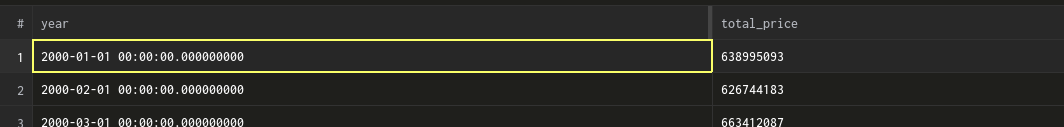
\includegraphics[width=150mm]{pricesumperyear-data.png}

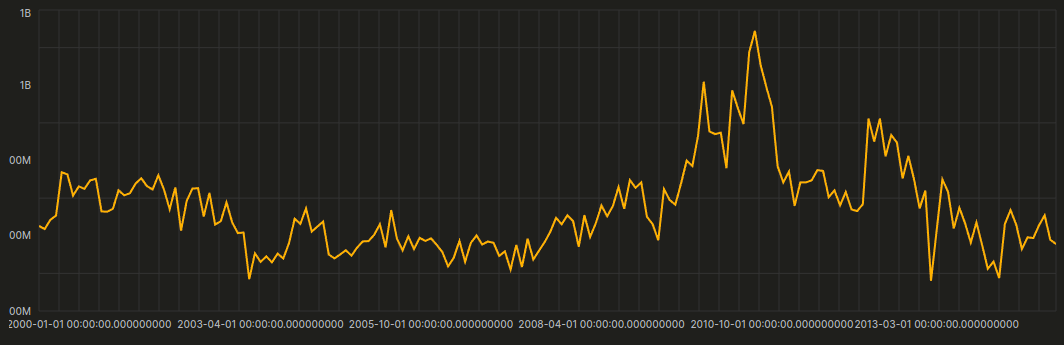
\includegraphics[width=150mm]{pricesumperyear.png}


\newpage
\section{20 nejvyšší cena bytů - rozděleno na města}

\begin{lstlisting}[
           language=SQL,
           showspaces=false,
           basicstyle=\ttfamily,
           commentstyle=\color{gray},
           keywordstyle=\color{cyan}
        ]
SELECT 
    td.year, ld.town, MAX(ft.resale_price) 
        AS highest_resale_price
FROM 
    FactTable AS ft
JOIN 
    Location_Dimension AS ld ON ft.LocationKey = ld.Index
JOIN 
    Time_Dimension AS td ON ft.TimeKey = td.Index
GROUP BY 
    td.year, ld.town
ORDER BY 
    highest_resale_price
LIMIT 20;
\end{lstlisting}

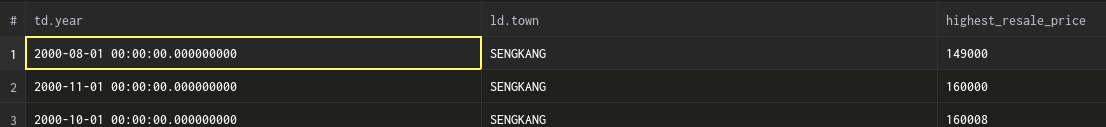
\includegraphics[width=150mm]{hvalpertown-data.png}

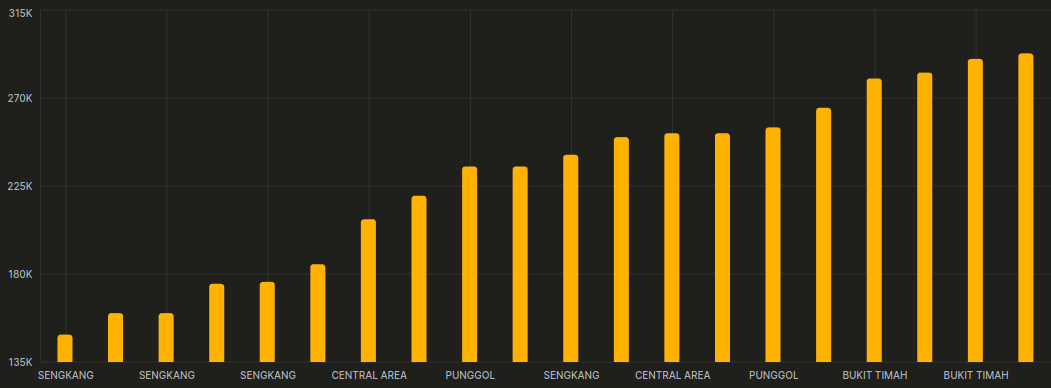
\includegraphics[width=150mm]{hvalpertown.png}


\newpage
\section{Průměrná cena bytů - rozděleno na města}

\begin{lstlisting}[
           language=SQL,
           showspaces=false,
           basicstyle=\ttfamily,
           commentstyle=\color{gray},
           keywordstyle=\color{cyan}
        ]
SELECT 
    l.town, AVG(f.resale_price) AS average_resale_price 
FROM 
    FactTable AS f 
JOIN 
    Location_Dimension AS l ON f.LocationKey = l.Index 
GROUP BY 
    l.town;
\end{lstlisting}

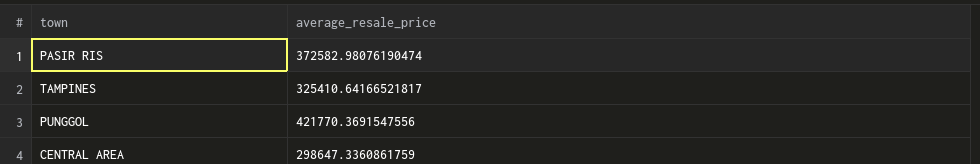
\includegraphics[width=150mm]{pricesumpertown-data.png}

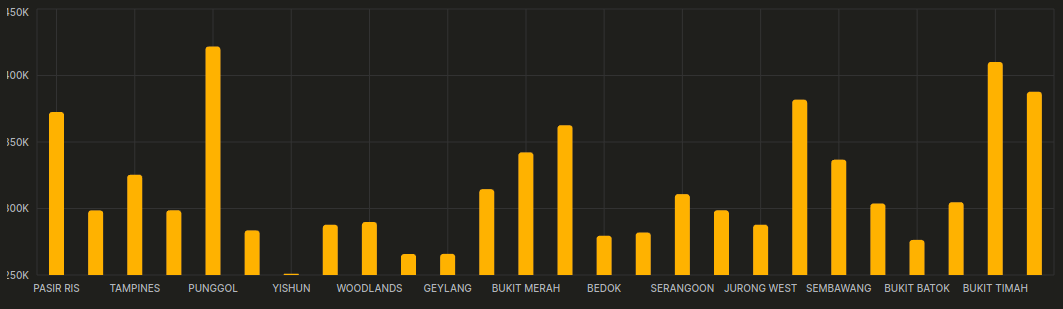
\includegraphics[width=150mm]{pricesumpertown.png}


\chapter{Data Mining}
Z toho co jsem dohledal tak ClickHouse neumožňuje využívat data mining metod, tedy jsem
se rozhodl tento krok vynechat a místo něj udělat 1 řez navíc.
\chapter{Závěr}
V rámci předmětu a vypracováním tohoto projektu, jsem pochopil využití OLAP databází. Dále jsem si zlepšil znalosti principů OLAP
databází a uplatnil načerpané znalosti ze seminářů v praxi. Troufnu si říct, že toto není naposled co
jsem usedal k OLAP databázím a v budoucím profesním životě se k ním jistě rád budu vracet. Nicméně stále nejsem dostatečně znalý OLAP systémů natolik, abych si troufl říct že je plně
ovládám, proto se jistě v rámci samostudia ještě k tomuto tématu navrátím.


%%% Seznam použité literatury
\nocite{*}
\printbibliography

\openright
\end{document}